\documentclass[a4paper, 12pt]{article}
\usepackage[slovene]{babel}
\usepackage[utf8]{inputenc}
\usepackage[T1]{fontenc}
\usepackage{hyperref}
\usepackage{graphicx}
\usepackage{wrapfig}
\usepackage[backend=bibtex]{biblatex}

\addbibresource{viri.bib}

\hypersetup{
colorlinks,
citecolor=black,
filecolor=black,
linkcolor=black,
urlcolor=black
}

\begin{document}

\begin{titlepage}
	\newcommand{\HRule}{\rule{\linewidth}{0.5mm}}
	\center

	\textsc{\LARGE Gimnazija Vič}\\[0.5cm]
	\textsc{\Large Tržaška c. 72, 1000 Ljubljana}\\[1.5cm]

	\HRule \\[0.4cm]
	{ \huge \bfseries Programiranje za mobilne platforme Android}\\[0.4cm]
	\HRule \\[1.5cm]

	\begin{minipage}{0.4\textwidth}
		\begin{flushleft} \large
			\emph{Avtor:}\\
			Žiga Patačko Koderman
		\end{flushleft}
	\end{minipage}
	~
	\begin{minipage}{0.4\textwidth}
		\begin{flushright} \large
			\emph{Mentor:} \\
			prof. Klemen Bajec
		\end{flushright}
		\end{minipage}\\[4cm]

		{\large \today}\\[3cm]

		\vfill
	\end{titlepage}

	\section*{Izvleček}
	[izvlecek placeholder]

	\section*{Abstract}
	[abstract placeholder]

	\pagebreak

	\tableofcontents
	\pagebreak

	\section{Uvod}
	\paragraph{}O morebitnih spremembah v organizaciji pouka in šolske prehrane je med šolskim letom treba sproti obveščati profesorje in dijake. Na Gimnaziji Vič so informacije o tem na voljo v spletni učilnici ter na oglasni deski v šoli. Ker pa sta oba načina pregledovanja nadomeščanj nekoliko zamudna, sem se že v prvem letniku odločil napisati aplikacijo za lažje pregledovanje teh podatkov kar na pametnem telefonu, ki jih večina dijakov in profesorjev v vsakdanjem življenju pogosto uporablja. Ker je med njimi največ takih z operacijskim sistemom Android\cite{android-wiki}, je aplikacija napisana za to platformo.  Zaradi pomankanja izkušenj se takrat problema še nisem lotil celovito. Aplikacijo sem zato kasneje še večkrat popravil in celo dvakrat napisal na novo. Razvoj zadnje različice 3.0 je opisan v tej seminarski nalogi.

\paragraph{} Preden sem se lotil razvoja aplikacije, sem si zadal določene cilje. Aplikacija GimVic 3.0 je morala dijakom in profesorjem Gimnazije Vič prikazovati urnik, nadomeščanja in jedilnik. Ker je javno objavljena, mora biti dostop do urnika zaradi varovanja zasebnosti po dogovoru z ravnateljico mag. Alenko Krapež za dijake omejen z največ petkratno izbiro razreda, za profesorje pa zaščiten z geslom. Ker aplikacija za delovanje potrebuje ažurne podatke, je za osvežitev podatkov nujna internetna povezava.

\paragraph{} Vsi zastavljeni cilji so bili tudi doseženi. Svojo uspešnost sem na koncu preveril še z obdelavo statističnih podatkov, pridobljenih z Googlove spletne strani za razvijalce.


	\section{Operacijski sistem Android}
	\paragraph{}Android je Googlov odprtokodni\cite{android-source} operacijski sistem mobilne naprave. Zgrajen je na Linuksovem jedru\cite{linux-kernel-wiki} in je bil prvotno namenjen uporabi na mobilnih telefonih. Kasneje se začel uporabljati tudi na tabličnih računalnikih, v zadnjem času pa celo na prenosnih računalnikih, urah in televizijah.

\subsection{Programiranje za platformo Android}
\paragraph{}Za razvoj aplikacij za platformo Android lahko uporabimo najrazličnejša razvijalska orodja, najpogosteje uporabljeno pa je Android Studio. Tega je razvilo podjetje Google in je osnovano na univerzalnem razvojnem orodju Intellij Idea\cite{intellij-idea} podjetja Jetbrains. Poleg platforme za razvoj aplikacij pa Google ponuja tudi spletno trgovino Google Play, kamor lahko razvijalci tudi objavimo svoje aplikacije.

\subsubsection{Programski jeziki}
\paragraph{}Za platformo Android lahko programiramo v več različnih jezikih, med njimi Java, Bash, C, C++ ter nekateri spletni jeziki (HTML, JavaScript, CSS), v zadnjem času pa celo Go in Python. Daleč najpogosteje se uporablja Java, saj je zanjo pripravljen zelo obširen nabor knjižnjic za interakcijo z uporabnikom ter cel kup orodji za prevajanje in sestavljanje posameznih delov v zaokroženo celoto imenovano aplikacija.

\subsubsection{Struktura aplikacije}
\paragraph{}Izvorna koda Android aplikacije je sestavljena iz več datotek in map. Te pa se delijo na 3 pomembnejše tipe:
\begin{itemize}
  \setlength\itemsep{0em}
  \item {\bf Manifest} datoteke so zapisane v formatu xml in operacijskemu sistemu povedo, kaj aplikacija počne, potrebuje, in zagotavljajo ostale podatke o njeni strukturi.
  \item {\bf Java} datoteke so izvorna koda v programskem jeziku Java, ki se izvaja na napravi.
  \item {\bf Res} ali {\bf resource} so datoteke, ki jih aplikacija potrebuje za prikazovanje uporabniškega vmesnika. To vključuje tekstovne datoteke xml, ki vsebujejo najrazličnejša besedila in opis izgleda aplikacije ter datoteke, ki vsebujejo slike, video posnetke in podobno gradivo.
\end{itemize}

\paragraph{}Med izvajanjem se aplikacija deli na posamezne niti. Vsaka nit opravlja svojo nalogo, ena iz med njih pa je glavna nit. Ta je prva, ki jo operacijski sistem požene in skrbi za zaganjanje ter ustavljanje vseh ostalih. Njena primarna naloga je skrb za uporabniški vmesnik. Zato ta nit ne sme opravljati nobenih dajših in zahtevnejših opravil, sicer aplikacija zastane, opracijski sistem pa jo zaradi tega po določenem času ubije.


	\section{Prejšnje različice}
	\paragraph{}Da bi aplikacija delovala kar najbolje in uporabnikom ponujala čim več podatkov, je njen razvoj do danes obsegal tri večje različice, vsaka med njimi pa tudi vrsto manjših sprotnih popravkov. Vsaka različica je korenito spremenila način pridobivanja, obdelovanja in prikazovanja podatkov.

\subsection{Različica 1.0}
\paragraph{}Prva različica aplikacije je prikazovala izključno nadomeščanja v preprosti besedilni obliki, ki jih je pridobila iz elektronske redovalnice Gimnazije Vič. Omogočala je osnovne filtre za posamezne razrede in omejen nabor filtrov za profesorje. Njeni glavni pomanjkljivosti sta bili:
\begin{itemize}
  \setlength\itemsep{0em}
  \item obdelava velike količine podatkov kar na mobilni napravi, zaradi česar je aplikacija delovala počasi in se včasih celo sesula,
  \item filtriranje z enim samim pogojem (razredom), kar pomeni, da uporabnik sploh ni mogel videti nadomeščanj za svoje izbirne predmete (to je veljalo predvsem za dijake višjih letnikov).
\end{itemize}

\subsection{Različica 2.0}
\paragraph{} Aplikacija GimVic 2.0 je sledila kakšno leto po svoji predhodnici. Da bi podatke o nadomeščanjih bolje umestili v kontekst, je ta verzija prikazovala celoten urnik z nadomeščanji. Izboljšan je bil tudi sistem filtriranja podatkov, ki je uporabniku omogočal prikazovanje njegovih izbirnih predmetov. Aplikacija pa je podatke še vedno obdelovala na telefonu. Teh je bilo zdaj še več, tako da so se na starejših napravah pojavljale težave s pomanjkanjem pomnilnika.

\subsection{Različica 3.0}
\paragraph{} Zadnja različica aplikacije je bila zasnovana z mislijo na dotedanje pomankljivosti. Podatki se obdelujejo na ločenem strežniku za vse uporabnike naenkrat, da se izognemo potratni in nepotrebni obdelavi podatkov na vsakem telefonu posebej. Poleg tega omogoča tudi prikazovanje jedilnika.


	\section{Razvoj in struktura aplikacije}
	\paragraph{}Ta projektna naloga se osredotoča na strukturo in razvoj zadnje različice aplikacije, verzije 3.0. Ta je objavljena na spletni trgovini Google Play na naslovu \url{https://play.google.com/store/apps/details?id=com.zigapk.gimvic.suplence}. Aplikacija je odprtokodna, njena izvorna koda pa je dostopna na spletnem portalu Github na naslovu \url{https://github.com/GimVic-app/gimvic-android/}.

\subsection{Pridobivanje podatkov}
\paragraph{}Aplikacija za svoje delovanje potrebuje podatke o:
\begin{itemize}
  \setlength\itemsep{0em}
  \item nadomeščanjih,
  \item urniku in
  \item jedilniku.
\end{itemize}

\paragraph{}Te se nahajajo na več različnih strežnikih v zelo različnih oblikah. Podatki o nadomeščanjih se pridobijo s spletne storitve elektronske redovalnice Gimnazije Vič v JSON\cite{json-wiki} (ang. \textit{JavaScript Object Notation}). Podatki o urniku za vse razrede in učitelje so na voljo na naslovu \url{http://old.gimvic.org/urnik/data.js}\cite{rin} v obliki izvorne kode JavaScript, ki generira tabelo. Sistem za pridobivanje podatkov o jedilniku pa je bilo treba še razviti.

\paragraph{}Posamezne jedilnike (več vrst malic in kosila) sestavlja na svojem računalniku organizatorica šolske prehrane ga. Eva Jelen v programu Excel. Da bi te podatke lahko dostavili in obdelali na strežniku, sem pripravil vtičnik za Excel, ki je dostopen na povezavi \url{https://github.com/GimVic-app/menu-uploader}. Ta je nameščen na njenem računalniku, tako da so lahko podatki o jedilnikih z enim klikom posodobljeni na spletnem strežniku.

\paragraph{}Da se izognemo nepotrebnemu in zahtevnemu obdelovanju podatkov na telefonu, je koncept delovanja zasnovan na sistemu strežnik - odjemalec. Na strežniku tečeta dva programa, ki mobilni aplikaciji zagotavljata željene podatke. To sta:
\begin{itemize}
  \setlength\itemsep{0em}
  \item posodobljevalnik podatkov in
  \item glavna strežniška aplikacija.
\end{itemize}

\paragraph{}Vsi zbrani podatki se v tej različici zberejo na strežniku in obdelajo ter shranijo v relacijsko podatkovno bazo MySQL\cite{mysql-wiki}. Temu je namenjen program Posodobljevalnik podatkov, dostopen na naslovu \url{https://github.com/GimVic-app/data-updater}. Podatki o urniku in nadomeščanjih se posodabljajo ob nastavljenih časovnih intervalih, podatki o jedilniku pa takoj, ko so posodobitve na voljo.

\paragraph{}Da lahko mobilna aplikacija  do podatkov v bazi dostopa prek interneta, je bilo potrebno napisati še glavno strežniško aplikacijo, ki prepozna uporabnikove nastavitve in na zahtevo mobilni aplikaciji postreže z željenimi podatki. Glavna strežniška aplikacija je napisana v programskem jeziku Go, njena izvorna koda pa je dostopna na naslovu \url{https://github.com/GimVic-app/server}.

\paragraph{}Mobilna aplikacija lahko tako s preprosto poizvedbo na strežnik dobi vse podatke v obliki JSON\cite{json-wiki}. Uporabnikove nastavitve aplikacija definira kar s parametri\cite{query-wiki} v URL naslovu. Podatki, ki jih strežnik vrne, vsebujejo seznam dni in za vsak dan natančno opisan urnik, morebitna nadomeščanja ter jedilnik.

\paragraph{}Celotna infrastruktura za pridobivanje, obdelavo in streženje podatkov je postavljena na strežniškem operacijskem sistemu Debian\cite{debian-wiki} različice 8 (\textit{Jessie}). Ta teče na virtualnem strežniku, ki ga je za potrebe aplikacije GimVic prijazno zagotovil Zavod 404 in je dostopen na spletnem naslovu \url{http://gimvicapp.404.si/}.

\subsection{Struktura aplikacije}
\paragraph{}Aplikacija je sestavljena iz več aktivnosti (ang. \textit{activities}). Najpomembnejše so:
\begin{itemize}
  \setlength\itemsep{0em}
  \item upravitelj podatkov,
  \item prikazovalnik podatkov,
  \item aktivnost za upravljanje z nastavitvami,
  \item aktivnost za izbiranje filtrov.
\end{itemize}

\subsubsection{Upravitelj podatkov}
\paragraph{}Upravitelj podatkov podaja informacije prikazovalniku podatkov. Te pridobiva v rednih intervalih s strežnika. V poizvedbah strežniku poda tudi uporabnikove nastavitve. Če glavna aktivnost potrebuje podatke, internetne povezave pa ni, upravitelj podatkov poda zadnje veljavne podatke, ki so shranjeni na napravi skupaj z datumom in časom zadnje posodobitve. Slednje je namenjeno uporabniku kot indikator ažurnosti podatkov.

\subsubsection{Prikazovalnik podatkov}
\paragraph{}Prikazovalnik podatkov (slika \ref{fig:main_activity}) uporabniku v obliki pregledne tabele izpiše njegov urnik ter jedilnik. Omogoča preprosto pomikanje med posameznimi dnevi v tednu ter vsebuje tudi povezavo do nastavitev. Podatke za prikazovanje dobi od upravitelja podatkov.

\subsubsection{Nastavitve}
\paragraph{}Nastavitve (slika \ref{fig:settings_activity}) omogočajo uporabniku nastavljanje vrste malice, kosila ter vklop oz. izklop prikazovanja nadomeščanj. Vsebujejo tudi gumb, ki uporabnika popelje na stran za izbiro razredov ter osnovne podatke o različici in avtorju aplikacije.

\subsubsection{Izbira filtrov}
\paragraph{}Aktivnost za izbiro filtrov (slika \ref{fig:filters_activity}) dijakom omogoča, da izberejo svoj razred in morebitne izbirne predmete, profesorjem pa, da izberejo svoj urnik. Po dogovoru z ravnateljico mag. Alenko Krapež je izbira razreda omejena na 5 sprememb, izbira profesorja pa zaščitena z univerzalnim profesorskim geslom.

% images
\begin{figure}[!htb]
\minipage{0.32\textwidth}
  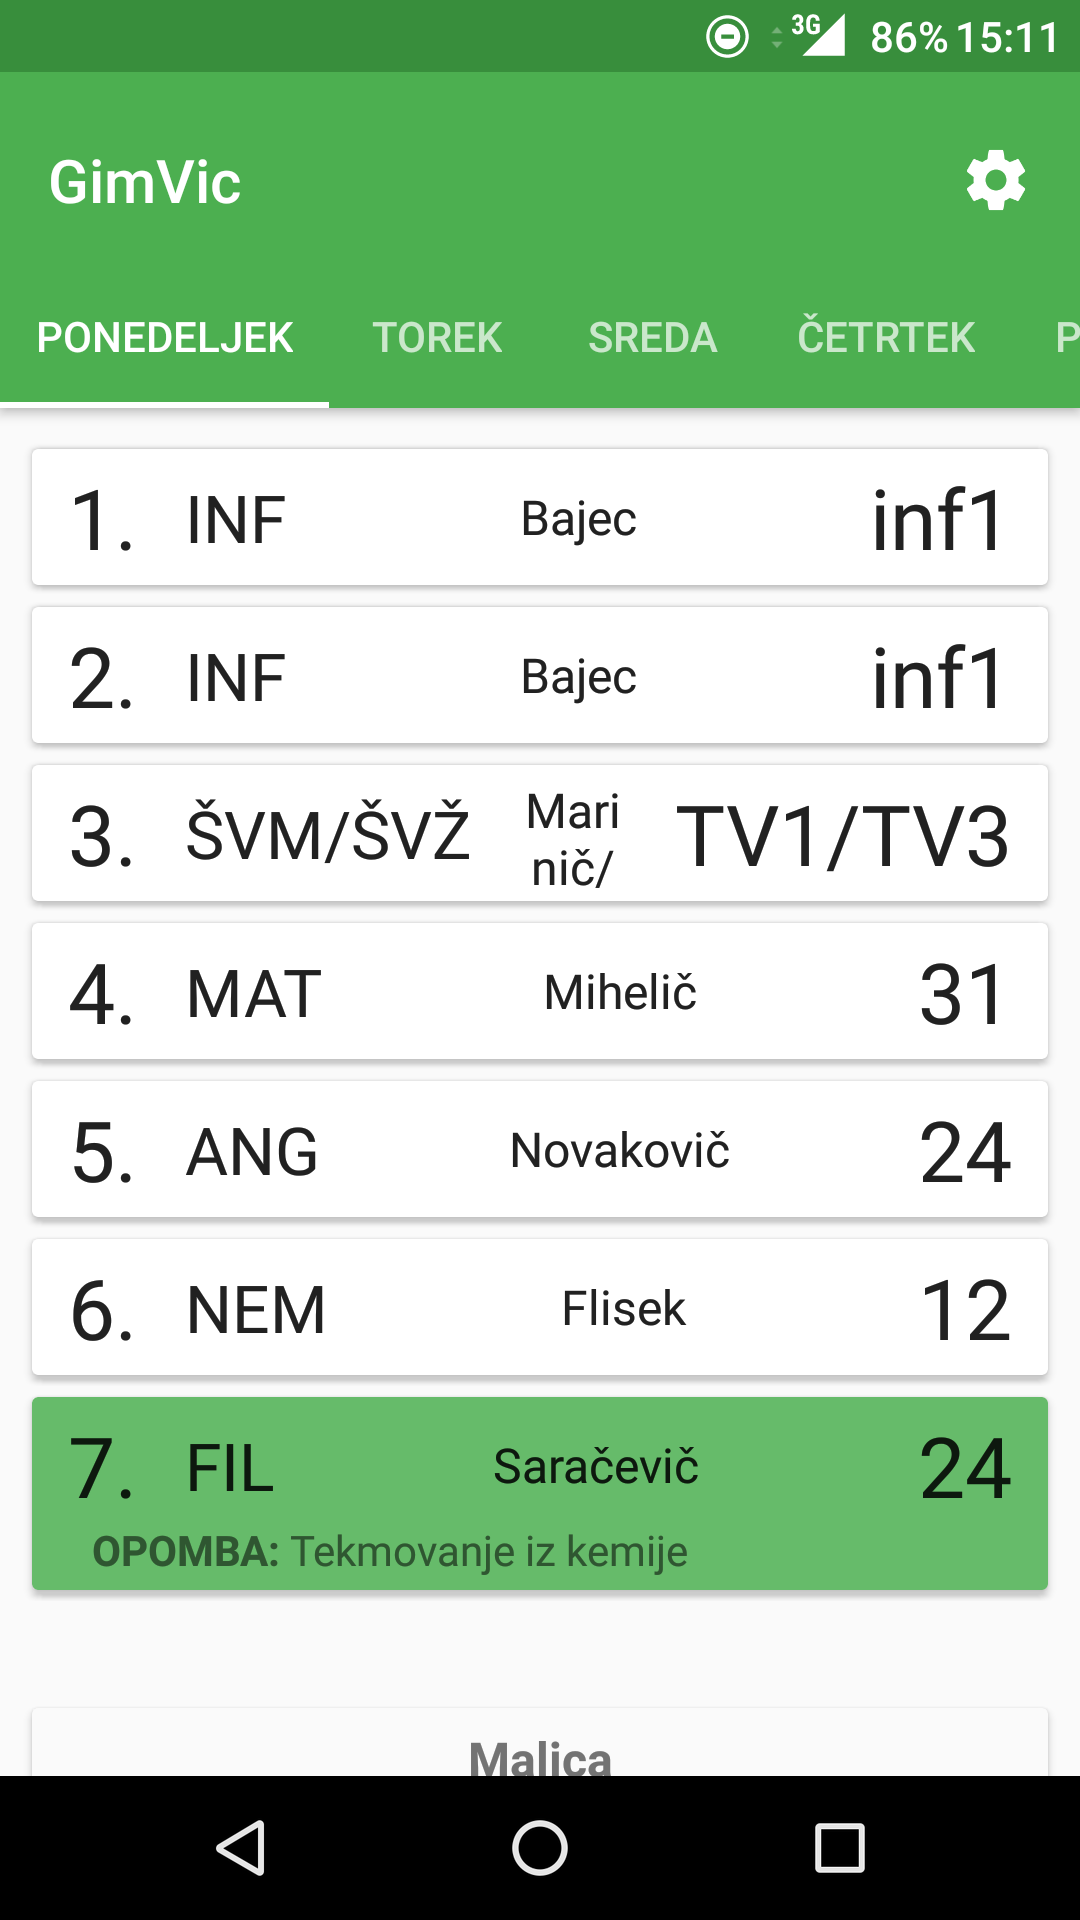
\includegraphics[width=\linewidth]{images/main.png}
  \caption{Glavna stran}\label{fig:main_activity}
\endminipage\hfill
\minipage{0.32\textwidth}
  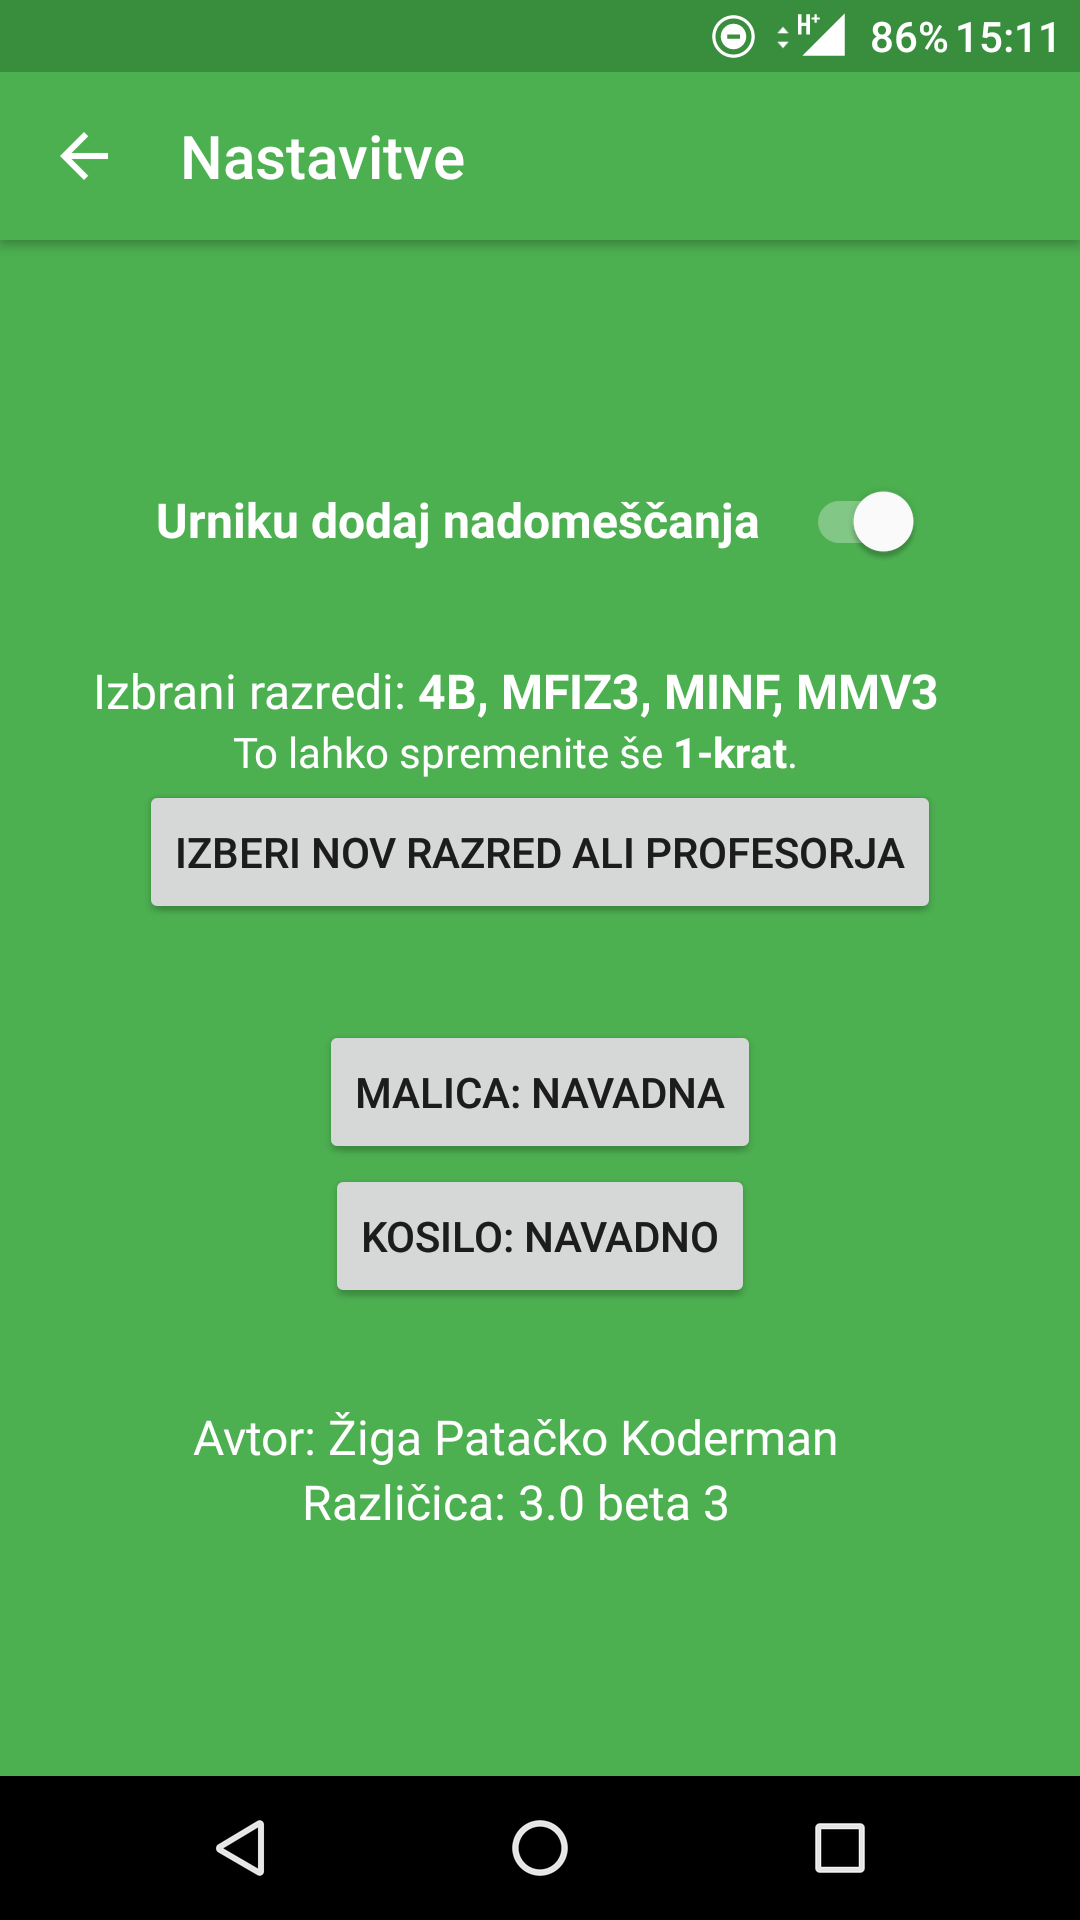
\includegraphics[width=\linewidth]{images/settings.png}
  \caption{Nastavitve}\label{fig:settings_activity}
\endminipage\hfill
\minipage{0.32\textwidth}%
  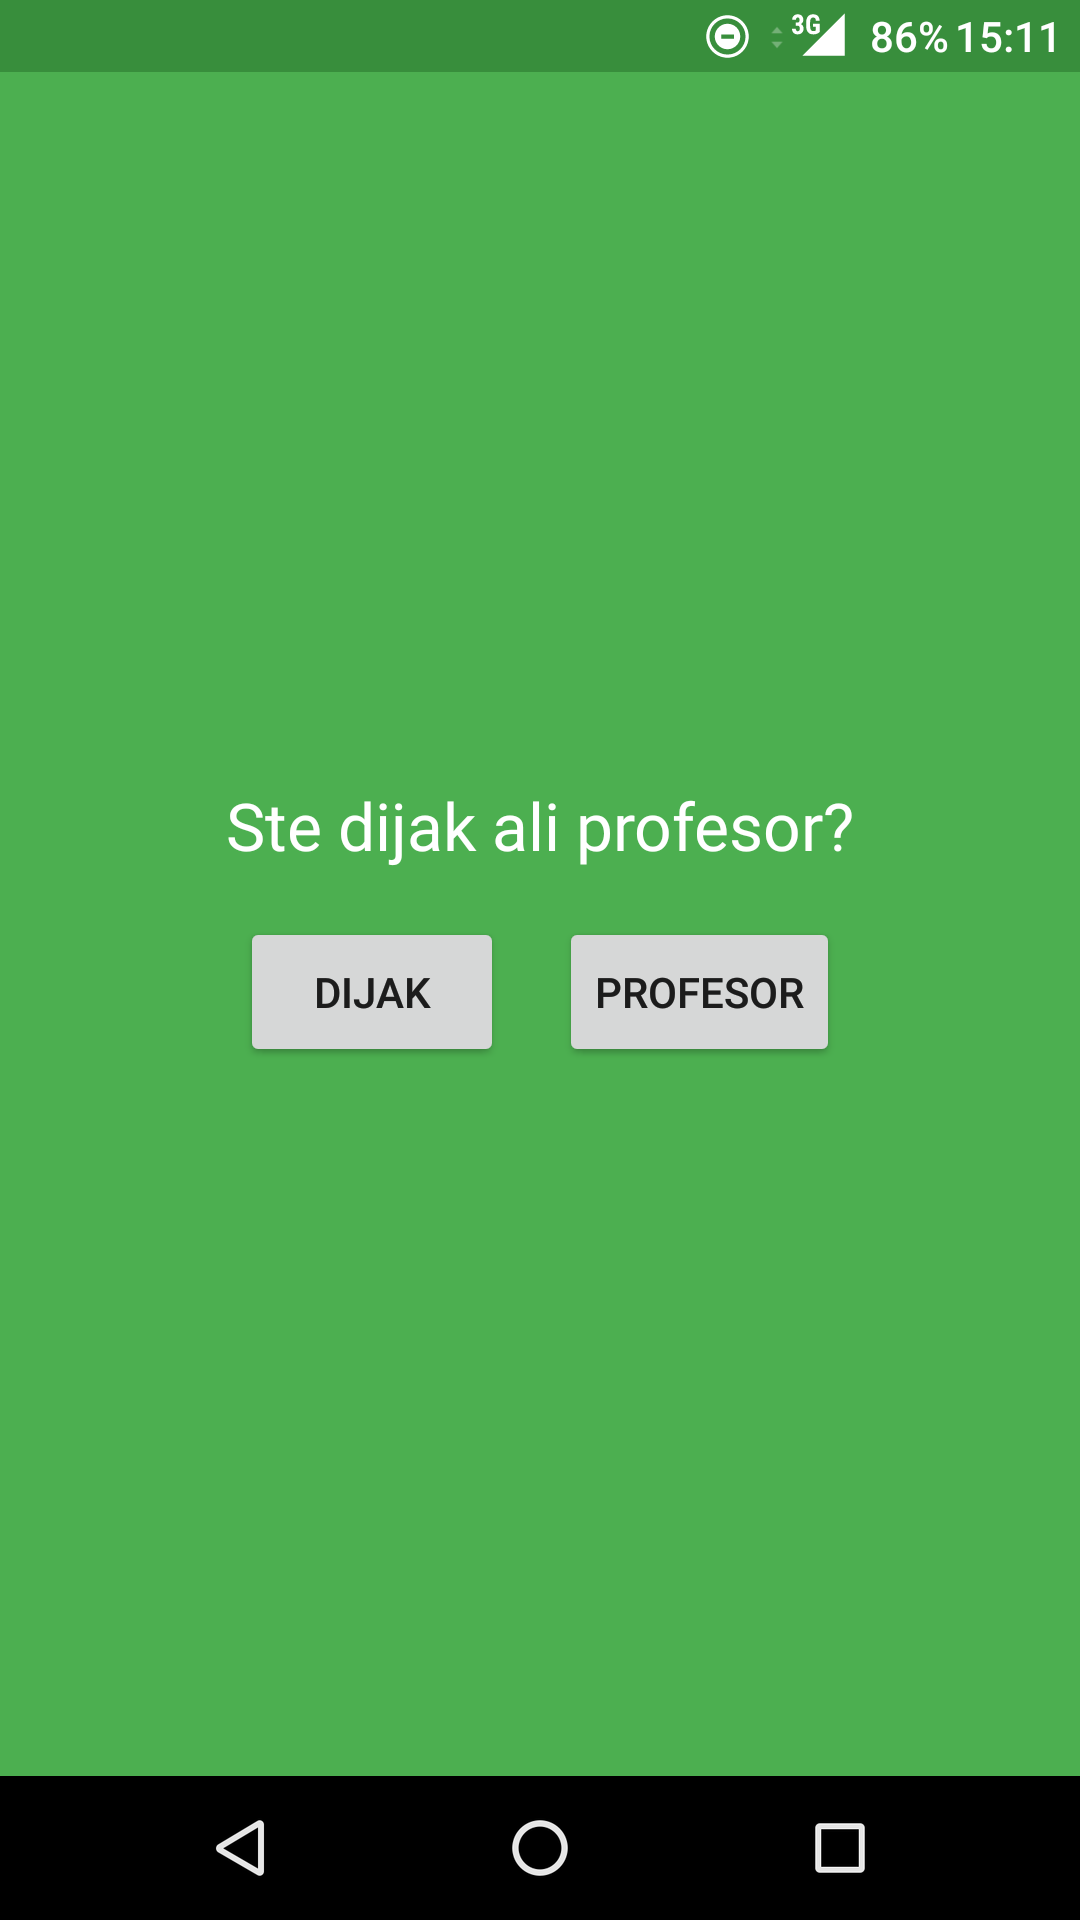
\includegraphics[width=\linewidth]{images/filters.png}
  \caption{Izbira filtrov}\label{fig:filters_activity}
\endminipage
\end{figure}


	\section{Objava aplikacije}

	\section{Odziv uporabnikov}

	\section{Zaključek}

	\pagebreak
	
	\printbibliography[heading=bibintoc]

	\end{document}
